\documentclass[10pt]{beamer}

% --- NOVO DESIGN ---
\usetheme{Berkeley} % Barra lateral para navegação constante
\usecolortheme{whale} % Base de cores sólidas
\useinnertheme{rounded} % Elementos internos arredondados

% Personalização de Cores Originais (Cinza Executivo e Dourado)
\definecolor{DeepSlate}{RGB}{37, 45, 51}
\definecolor{GoldAccent}{RGB}{191, 161, 98}

\setbeamercolor{palette primary}{bg=DeepSlate, fg=white}
\setbeamercolor{palette secondary}{bg=DeepSlate!90, fg=white}
\setbeamercolor{sidebar}{bg=DeepSlate} % Cor da barra lateral
\setbeamercolor{title}{fg=DeepSlate, bg=GoldAccent!20}
\setbeamercolor{frametitle}{fg=DeepSlate, bg=white}
\setbeamercolor{structure}{fg=DeepSlate} % Cor de listas e títulos
\setbeamercolor{section in sidebar}{fg=GoldAccent} % Destaque na lateral
\setbeamercolor{block title}{bg=DeepSlate, fg=white}
\setbeamercolor{block body}{bg=DeepSlate!5, fg=black}

% Fontes e pacotes
\usepackage[utf8]{inputenc}
\usepackage[T1]{fontenc}
\usepackage{graphicx}
\usepackage{booktabs}
\usepackage{amsmath}
\usepackage{tikz}
\usepackage{pgfplots}
\pgfplotsset{compat=1.18}

% Remove os símbolos de navegação inúteis no canto inferior
\setbeamertemplate{navigation symbols}{}

% Informações
\title{Apresentação de Teste}
\subtitle{Exemplo com Design Customizado}
\author{Autor Exemplo}
\institute{Instituição Exemplo}
\date{\today}

\begin{document}

% Slide 1 - Capa (Design diferente com logo na lateral)
\begin{frame}[plain] % plain remove a barra lateral na capa para foco total
    \titlepage
\end{frame}

% Slide 2 - Sumário
\section*{Início}
\begin{frame}{Plano de Voo}
    \tableofcontents
\end{frame}

% Slide 3 - Introdução
\section{Introdução}
\begin{frame}{Introdução}
    Esta é uma apresentação de teste criada em \LaTeX\ utilizando o pacote \textbf{Beamer}.  
    \vspace{0.3cm}
    \begin{itemize}
        \item Note como a barra lateral ajuda na orientação.
        \item O design agora é focado na leitura vertical.
    \end{itemize}
\end{frame}

% Slide 4 - Texto e Parágrafo
\begin{frame}{Texto e Parágrafo}
    O \LaTeX\ é amplamente utilizado para produção de documentos científicos, pois oferece alta qualidade tipográfica.
    
    \vspace{0.5cm}
    \setbeamercolor{postit}{fg=black,bg=GoldAccent!30}
    \begin{beamercolorbox}[sep=0.3em,wd=10cm]{postit}
        Diferente do Word, aqui o foco é o conteúdo estruturado.
    \end{beamercolorbox}
\end{frame}

% Slide 5 - Lista Simples
\begin{frame}{Lista Simples}
    \begin{itemize}
        \item Alta qualidade tipográfica
        \item Organização estrutural
        \item Facilidade com matemática
        \item Uso acadêmico e profissional
    \end{itemize}
\end{frame}

% Slide 6 - Lista Enumerada
\begin{frame}{Lista Enumerada}
    \begin{enumerate}
        \item Introdução
        \item Desenvolvimento
        \item Resultados
        \item Conclusão
    \end{enumerate}
\end{frame}

% Slide 7 - Matemática
\section{Matemática}
\begin{frame}{Fórmula Matemática}
    A famosa equação da relatividade é dada por:
    \begin{equation*}
        E = mc^2
    \end{equation*}
    Onde $E$ é a energia, $m$ a massa e $c$ a velocidade da luz.
\end{frame}

% Slide 8 - Fórmula Avançada
\begin{frame}{Equação Mais Elaborada}
    \[
        \int_{a}^{b} f(x)\,dx = F(b) - F(a)
    \]
    \centering
    \textit{Teorema Fundamental do Cálculo.}
\end{frame}

% Slide 9 - Bloco de Destaque
\begin{frame}{Bloco de Informação}
    \begin{block}{Definição de Função}
        Uma função é uma relação que associa cada elemento de um conjunto a exatamente um elemento de outro conjunto.
    \end{block}
\end{frame}

% Slide 10 - Citação
\section{Citações}
\begin{frame}{Citação}
    \begin{quote}
        ``A matemática é a linguagem com a qual Deus escreveu o universo.''  
        \hfill — Galileu Galilei
    \end{quote}
\end{frame}

% Slide 11 - Tabelas
\section{Tabelas}
\begin{frame}{Tabela Simples}
    \centering
    \begin{tabular}{l r r}
        \toprule
        \textbf{Item} & \textbf{Valor A} & \textbf{Valor B} \\
        \midrule
        A & 10 & 20 \\
        B & 15 & 25 \\
        C & 30 & 40 \\
        \bottomrule
    \end{tabular}
    \caption{Exemplo de tabela estilizada}
\end{frame}

% Slide 12 - Tabela Comparativa
\begin{frame}{Tabela Comparativa}
    \centering
    \begin{tabular}{|l|c|}
        \hline
        \textbf{Tecnologia} & \textbf{Popularidade} \\ \hline
        LaTeX & Alta \\ \hline
        Word & Muito Alta \\ \hline
        Markdown & Média \\ \hline
    \end{tabular}
\end{frame}

% Slide 13 - Gráficos
\section{Gráficos}
\begin{frame}{Gráfico de Barras}
    \centering
    \resizebox{0.7\textwidth}{!}{
    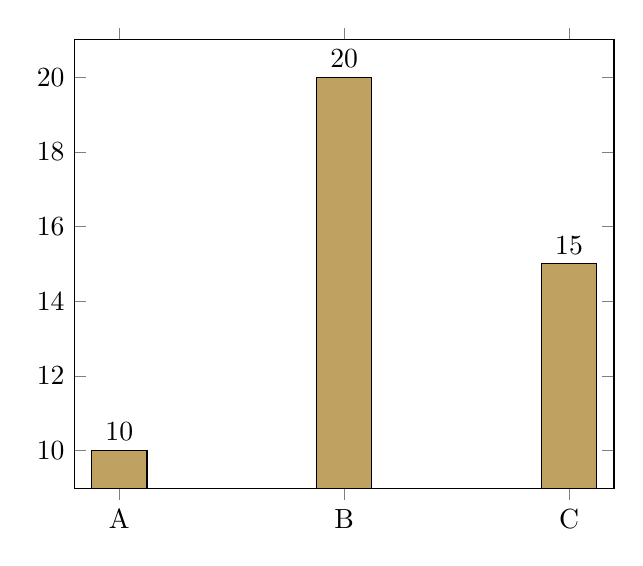
\begin{tikzpicture}
    \begin{axis}[
        ybar,
        symbolic x coords={A,B,C},
        xtick=data,
        nodes near coords,
        bar width=20pt,
    ]
    \addplot[fill=GoldAccent] coordinates {(A,10) (B,20) (C,15)};
    \end{axis}
    \end{tikzpicture}
    }
\end{frame}

% Slide 14 - Gráfico de Linha
\begin{frame}{Gráfico de Linha}
    \centering
    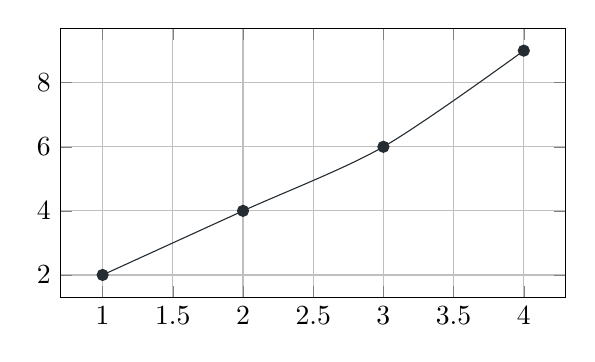
\begin{tikzpicture}
    \begin{axis}[grid=major, width=8cm, height=5cm]
    \addplot[smooth, mark=*, DeepSlate] coordinates {(1,2) (2,4) (3,6) (4,9)};
    \end{axis}
    \end{tikzpicture}
\end{frame}

% Slide 15 - Combinações
\section{Combinações}
\begin{frame}{Texto e Matemática}
    O crescimento exponencial pode ser modelado por:
    \[
        f(x) = a \cdot e^{bx}
    \]
    Design limpo para melhor foco no conteúdo.
\end{frame}

% Slide 16 - Alerta
\begin{frame}{Alerta}
    \begin{alertblock}{Atenção}
        A barra lateral à esquerda ajuda o público a saber exatamente onde você está na apresentação.
    \end{alertblock}
\end{frame}

% Slide 17 - Elementos Visuais
\section{Visual}
\begin{frame}{Forma Geométrica}
    \centering
    
\begin{tikzpicture}
        \draw[GoldAccent, ultra thick] (0,0) circle (1cm);
        \node at (0,0) {Foco};
    \end{tikzpicture}
\end{frame}

% Slide 18 - Conclusão
\section{Conclusão}
\begin{frame}{Conclusão}
    O Beamer com tema lateral oferece uma experiência de navegação superior para apresentações longas.
\end{frame}

% Slide 19 - Considerações Finais
\begin{frame}{Considerações Finais}
    \begin{itemize}
        \item[$\checkmark$] Visual Profissional
        \item[$\checkmark$] Navegação Intuitiva
        \item[$\checkmark$] Cores sóbrias
    \end{itemize}
\end{frame}

% Slide 20 - Encerramento
\begin{frame}[plain]
    \centering
    \Huge \textcolor{DeepSlate}{Obrigado!} \\
    \vspace{0.8cm}
    \Large Perguntas?
\end{frame}

\end{document}